\documentclass[
    11pt,
    a4paper,
    egregdoesnotlikesansseriftitles,
    toc=chapterentrywithdots,
    twoside,openright,
    titlepage,
    parskip=half,
    headings=normal,  % reduces heading size
    listof=totoc,
    bibliography=totoc,
    index=totoc,
    captions=tableheading,  % caption below table
    chapterprefix,
    listof=flat,
    final
]{scrbook}


% details about your thesis
\newcommand{\titel}{Abstractive Text Summarization of Meetings}
\newcommand{\artderarbeit}{Bachelorarbeit}  % {Bachelorarbeit,Masterarbeit}
\newcommand{\autor}{Bastian Oppermann}
\newcommand{\studiengang}{Informatik}  % {Informatik,Wirtschaftsinformatik,Medieninformatik}
\newcommand{\matrikelnr}{3068074}
\newcommand{\erstgutachter}{Prof.\,Dr.~Korbinian Riedhammer}
\newcommand{\zweitgutachter}{Prof.\,Dr.~Ngoc\,Thang\,Vu}
\newcommand{\logo}{figures/TH-Nuernberg-RGB.png}
\newcommand{\keywords}{bert, summarization}
 

% custom head and foot
\usepackage[automark]{scrlayer-scrpage}
\pagestyle{scrheadings}
\ihead{\headmark}
\chead{}
\ohead{\pagemark}
\renewcommand*\chaptermarkformat{\chapappifchapterprefix{\ }% 
  \thechapter.\enskip}

\RedeclareSectionCommand[tocindent=0pt]{section}
\RedeclareSectionCommand[tocindent=0pt]{subsection}
%\RedeclareSectionCommand[tocnumwidth=70pt]{chapter}

\usepackage{scrhack}

% other packages
\usepackage[utf8]{inputenc}
\usepackage[T1]{fontenc}
\usepackage{lmodern,relsize,textcomp,csquotes}
\usepackage{amsmath,amsfonts}
\usepackage[ngerman,english]{babel}  % flip for German thesis
\usepackage[final]{graphicx}
\usepackage{setspace,geometry,xcolor}
\usepackage{makeidx}
\usepackage{paralist,ifthen,todonotes}
\usepackage{url}
\usepackage{pdfpages}

% table setup
\usepackage{longtable}
\usepackage{array}
\usepackage{ragged2e}
\usepackage{lscape}

% pdf hyperref
\usepackage[
    bookmarks=true,
    bookmarksopen=true,
    bookmarksnumbered=true,
    bookmarksopenlevel=1,
    pdftitle={\titel},
    pdfauthor={\autor},
    pdfcreator={\autor},
    pdfsubject={\titel},
    pdfkeywords={\keywords},
    pdfpagelabels=true,
    colorlinks=true,
    linkcolor=red,
    urlcolor=magenta,
    anchorcolor=black,
    citecolor=cyan,
    filecolor=magenta,
    menucolor=red,
    plainpages=false,
    hypertexnames=true,
    linktocpage=true,
]{hyperref}


% configure your listings style
\usepackage{listings}
\lstset{
	tabsize=3,
	extendedchars=true,
	frame=single,
	showstringspaces=true,
	numbers=left,
	numberstyle=\small,
	breakautoindent=true
}

% page setup
% \setlength{\topskip}{\ht\strutbox}
\geometry{paper=a4paper,left=2.5cm,top=3.0cm,bindingoffset=.8cm}
\onehalfspacing
\frenchspacing
\clubpenalty = 10000
\widowpenalty = 10000 
\displaywidowpenalty = 10000

% some commands
\newcommand{\ua}{\mbox{u.\,a.\ }}
\newcommand{\zB}{\mbox{z.\,B.\ }}
\newcommand{\dahe}{\mbox{d.\,h.,\ }}
\newcommand{\bzw}{\mbox{bzw.\ }}
\newcommand{\bzgl}{\mbox{bzgl.\ }}
\newcommand{\eg}{\mbox{e.\,g.\ }}
\newcommand{\Eg}{\mbox{E.\,g.\ }}
\newcommand{\ie}{\mbox{i.\,e.\ }}
\newcommand{\wrt}{\mbox{w.\,r.\,t.\ }}
\newcommand{\etal}{\mbox{\emph{et.\,al.\ }}}


% TODO remove if not needed...
\usepackage{blindtext}


\begin{document}

\setcounter{secnumdepth}{3}  % numerate subsections
\setcounter{tocdepth}{2}  % ...but don't include them in toc

\frontmatter
\thispagestyle{empty}
\pdfbookmark[1]{Cover}{cov}
\begin{titlepage}

\begin{center}


\includegraphics[width=\linewidth]{figures/TH-Nuernberg-RGB.png}\\[1cm]
\LARGE{Fakultät Informatik}\\[2cm]

\huge
\textbf{\titel}\\[1cm]
%
\Large
\artderarbeit~im Studiengang \studiengang\\[1cm]
%
\large
vorgelegt von

\Large
\autor\\[0.5cm]
\small
Matrikelnummer \matrikelnr\\[2cm]

\vspace*{\fill}

\large
\begin{tabular}{p{3cm}p{8cm}}\\
Erstgutachter:  & \quad \erstgutachter\\[1.2ex]
Zweitgutachter: & \quad \zweitgutachter
\end{tabular}
\end{center}

\begin{center}
\copyright\,\the\year
\end{center}

\vspace{-0.5cm}
\singlespacing
\small
\noindent Dieses Werk einschließlich seiner Teile ist \textbf{urheberrechtlich geschützt}.
Jede Verwertung außerhalb der engen Grenzen des Urheberrechtgesetzes ist ohne Zustimmung des Autors unzulässig und strafbar.
Das gilt insbesondere für Vervielfältigungen, Übersetzungen, Mikroverfilmungen sowie die Einspeicherung und Verarbeitung in elektronischen Systemen.

\end{titlepage}
\cleardoublepage

% download the following form and complete it (hit save in your editor)
% https://intern.ohmportal.de/fileadmin/Gelenkte_Doks/Abt/SZS/SB/SB_0050_FO_Pruefungsrechtliche_Erklaerung_und_Erklaerung_zur_Veroeffentlichung_der_Abschlussarbeit_public.pdf
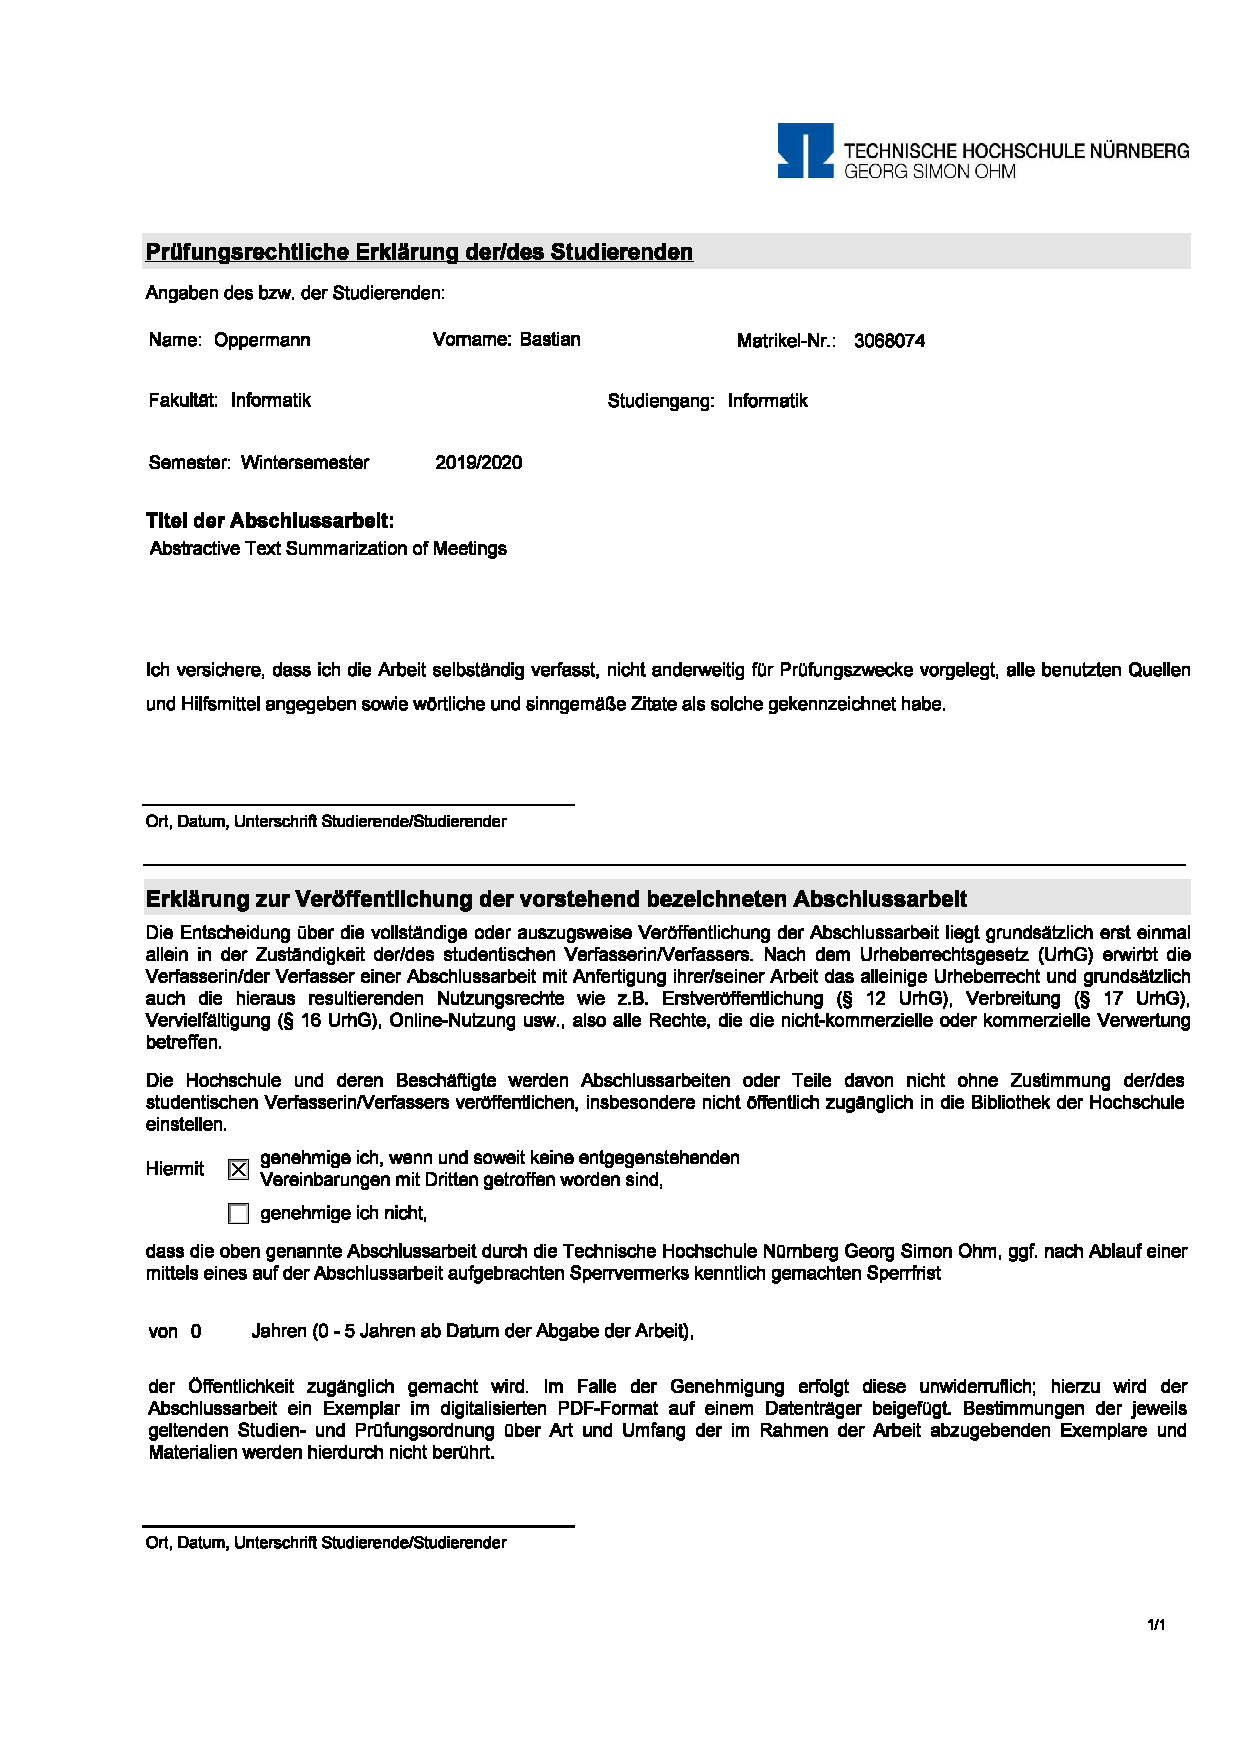
\includepdf{SB_0050_FO_Pruefungsrechtliche_Erklaerung_und_Erklaerung_zur_Veroeffentlichung_der_Abschlussarbeit_public.pdf}\cleardoublepage

\thispagestyle{empty}
\section*{Kurzdarstellung}
\label{sec:kurzdarstellung}

Die vorliegende Bachelorarbeit untersucht, wie ein modernes vortrainiertes neuronales Netz, wie z.B. Googles BERT \cite{devlin2018bert}, zur abstrakten Textzusammenfassung von Meetings genutzt werden kann.

Im Rahmen dieser Arbeit wird ein Tranformer Netz \cite{1706.03762} implementiert, das BERT als seinen Encoder nutzt.
Der Decoder des Netzes ist ein normaler, nicht vortrainierter, Transormer-Decoder.
Das Netz wird hierfür mit Daten aus dem AMI Meeting Corpus \cite{Mccowan05theami} und dem ICSI Meeting Corpus \cite{Janin} trainiert.
Es wird dafür ein 2-stufiges Verfahren genutzt.
Im ersten Schritt wird das Netzwerk darauf trainiert, eine Menge von Dialogen auf einen einzelnen Satz abzubilden, der aus der abstrakten Zusammenfassung des Meetings stammt.
Im zweiten Schritt werden die Meetings nach Themen aufgeteilt und anschließend alle Dialoge eines Themas als Eingabe für das neuronale Netz genutzt.
Die zusammengehängte Ausgabe des Netzes für alle Themen eines Meetings ist dann die fertige Zusammenfassung des gesamten Meetings.
Dies dient zum einen dazu, den benötigten Speicherbedarf von BERT bei langen Textsequenzen zu reduzieren.
Zum anderen kann damit auch das Problem umgangen werden, dass BERT nur mit Textsequenzen bis zu einer Länge von 512 vortrainiert wurde \cite[p.~13]{devlin2018bert}.

Die Arbeit zeigt, dass ein datengetriebener Ansatz in der Theorie funktioniert.
Allerdings haben die Ergebnisse eine sehr starke Neigung dazu, Informationen aus den Traingsdaten in die Zusammenfassung einfliesen zu lassen, selbst wenn diese nicht in der Eingabe vorhanden sind.
Dies ist besonders offensichtlich, wenn ein Netz, das nur mit dem AMI Korpus trainiert wurde, auf den ICSI Corpus angewendet wird.
Die hierbei erziehlten Ergebnisse sind meist sehr schlecht.
Hieraus lässt sich ableiten, dass wesentlich mehr Trainigsdaten notwendig sind, um praxistaugliche Ergebnisse zu erzielen, die unabhängig von einem stark eingegrenzten Kontext, wie es bei den AMI Szenario-Meetings der Fall ist, sind.


\section*{Abstract}
\label{sec:abstract}

This work analyzes how a state-of-the-art pretrained neural network - such as Google's BERT \cite{devlin2018bert} - can be fine-tuned to the task of abstractive text summarization in the context of meetings.

As part of this work a Transformer network \cite{1706.03762} is developed, that uses BERT as its encoder and a plain decoder.
It is trained on the AMI Meeting Corpus \cite{Mccowan05theami} as well as the ICSI Meeting Corpus \cite{Janin}.
To circumvent the high memory usage of BERT at long sequence lengths and the fact that BERT is pre-trained with a maxiumum sequence length of 512 \cite[p.~13]{devlin2018bert}, the summarization is performed using a two-step approach.
First, the network is trained to summarize \(n\) dialouge acts to a single sentence of the meeting's abstractive summary.
Afterwards, a whole meeting is split by its topics and all the dialouge acts of a topic are fed into the trained network as its input.
The concatenated outputs of the Transformer for every topic is the final summary.

The work proofs, that a data-driven approach is feasible in theory.
However, the results have a strong bias towards the context of the meeting and cross-corpus validation on AMI and ICSI shows a very poor performance.
This indicates, that far more training data is necessary for practicable results outside of a very topic-specific context like the scenario meetings of the AMI corpus. \cleardoublepage

\tableofcontents

\mainmatter
\chapter{Introduction}\label{ch:Introduction}

% Motivation

Transfer Learning is known to improve results on many different machine learning tasks.
Google's recently announced language representation model BERT broke records for many Natural Language Processing benchmarks \cite[p.~5--7]{devlin2018bert}, such as  SQuAD v1.1 \cite{rajpurkar-etal-2016-squad} or GLUE \cite{1804.07461}.
There have been some attempts to apply BERT to the problem of abstractive summarization, like \cite{1902.09243} and \cite{1908.08345}.
However, they are usually trained and tested on news articles.
Generating abstractive summaries of meetings is only a rarely researched topic.
Most of the research for summarizing meetings has been focused on either extractive summarization or non Deep Learning approaches such as Dependency Graph Fusion \cite{1609.07035} or Multi-Sentence Compression \cite{shang-etal-2018-unsupervised}.

% ==============
% PROBLEM DEFINITION
% ==============

\section{Problem Definition}

The goal of this work is to analyze, if a data driven approach is feasible for abstractive meeting summarization.
Transfer Learning should be used to compensate for the small amount of training data that is available for meeting summarization.
As BERT's pre-training sequence length of 512 \cite[p.~13]{devlin2018bert} is way shorter than a typical meeting, a method should be developed that deals with this limitation.

% ======
% METHOD
% ======

\section{Method}

As part of this work, a network is developed that uses BERT.
It is trained with data from the two most commonly used meeting corpora, the AMI Meeting Corpus \cite{Mccowan05theami} and the ICSI Meeting Corpus \cite{Janin} that are described in \autoref{ch:used-corpora}.
Cross-corpus validation\footnote{\Eg training on the ICSI corpus and testing on the AMI corpus} is performed to evaluate if the network is able to generalize what it learned.

% =================
% STRUCTURE OF THE WORK
% =================

\section{Structure of the work}

Chapter \ref{ch:theoretical-foundation} explains the theoretical foundation that is necessary for this work.
Chapter \ref{ch:used-corpora} introduces the two used meeting corpora.
Chapter \ref{ch:concept} explains the concept of the model that this works uses.
It will also present how the model is trained.
Chapter \ref{ch:implementation} focuses on the implementation if the model and how the training data is processed.
Chapter \ref{ch:results} presents the results. It shows both the archived scores and provide some hand-picked example outputs.
Chapter \ref{ch:outlook} gives an outlook for possible future research.
Finally, chapter \ref{ch:summary-and-conclusion} summarizes the results of the work and draws a conclusion how they can be interpreted.

\chapter{Theoretical Foundation }\label{ch:theoretical-foundation}

\Blindtext

% ===========
% DEEP LEARNING
% ===========

\section{Deep Learning}

\Blindtext

% ==========
% TRANSFORMER
% ==========

\section{Transformer}

The Transformer is a neural network architecture for sequence learning that was published in 2017 \cite{1706.03762}.
It achived new state-of-the-art results for many machine translation tasks while at the same time requiring significat less training time compared to previous well performing models.

\subsection{Motivation}

In the recent years, recurrent neural networks (RNNs) have been the most common way to solve sequence learning tasks.
One of the big downsides of RNNs is its sequential behaviour.
To train a RNN, the elements of the input sequence is fed into the neural network one after another.
While the sequence elements are passed through the RNN, a hidden state gets computed at every step, that is part of the input for the next step.
This process is called encoding.
Afterwards, the last hidden state of the econding process is used as an input for the first step of the decoding process.
Because of this, it is not possible to parallelize the training within a training example, as the hidden state of the previous step is needed to calculate the output of the current step. \cite[p.~~2]{1706.03762}
A simplified RNN for sequence-to-sequence tasks like machine translation is shown in \autoref{fig:rnn-visualisation}.

\begin{figure}[h]
\centering
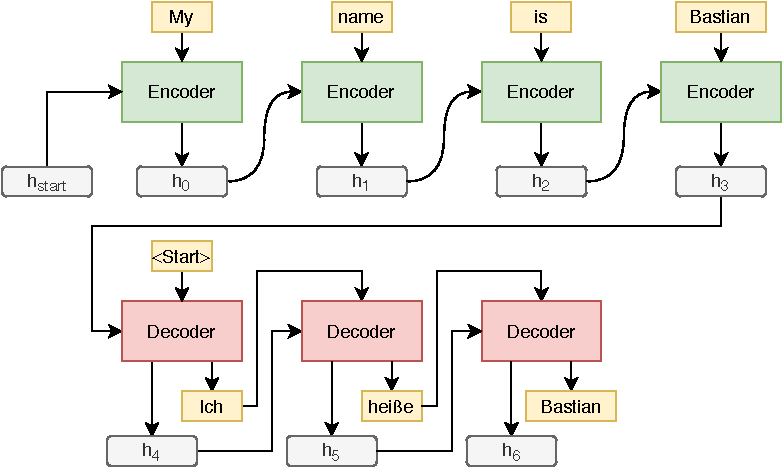
\includegraphics{figures/rnn-visualisation}
\caption{Simplified visualisation of a sequence-to-sequence RNN network for machine translation. The input sequence is fed into the Encoder with one word each step. The final hidden state, that is computed in the last encoding step, is used as input for the first decoding step. The initial hidden state $h_{start}$ can be initialized as a vector of zeros or learned during training.}
\label{fig:rnn-visualisation}
\end{figure}

Another problem of RNNs is the long distance, information has to "travel" before it is used.
Information that was encoded into the hidden state has to pass through multiple encoding and decoding steps, before it is finally used in one of the decoding steps.
Besides having the hidden state as an information bottleneck, this also makes it very hard for the network to learn long range dependencies because of the problem of vanishing or explosing gradients \cite{Hochreiter01gradientflow}.
Modern variants of RNNs like the long short-term memory (LSTM) architecture \cite{Hochreiter1997} try to mitigate these effects, but aren't able to fully elliminate them.
A fairly recent solution to this problem is the attention mechanism, that was first proposed in 2014 \cite{1409.0473}.
It allows the network in the decoding stage to retrieve information from any hidden state that was computed during the encoding stage.
This eliminates the problem of learning long range dependencies.

The Transformer network tries to take advantage of the attention mechanism while ditching the recurrence of RNNs to achieve faster training and allowing for more parallelization.

\subsection{Model Architecture}

\Blindtext

\subsection{Difference to RNNs}

\Blindtext

\subsection{Advantages}

\Blindtext

\subsection{Disadvantages}

\Blindtext

% ====
% BERT
% ====

\section{BERT}

BERT (\textbf{B}idirectional \textbf{E}ncoder \textbf{R}epresentations from \textbf{T}ransformers) is a general-purpose language model, that was released by Google AI researchers in mid 2018.
It broke several records for Natural Language Processing Benchmarks \cite[p.~5--7]{devlin2018bert}, such as  SQuAD v1.1 \cite{rajpurkar-etal-2016-squad} or GLUE \cite{1804.07461}.

\subsection{Motivation}

It has been shown, that results for many natural language processing tasks can be improved with the help of language models.
The most famous amoung them are OpenAI's GPT-2 \cite{radford2019language} and ELMo \cite{1802.05365}.
The benefit of language models is, that most of them can be trained on unlabeled data, like Wikipedia articles or large book corpora.
This allows them to learn from a huge amount of data, as there is no need for time-consuming labeling of the training data and any texts can be used.
By pre-training them on normal texts, the networks can get a general sense of natural language.
This general sense for language can then be used for more specific tasks.

% TODO Not sure if I keep using this or create an own one / just remove it
\begin{figure}[h]
\centering
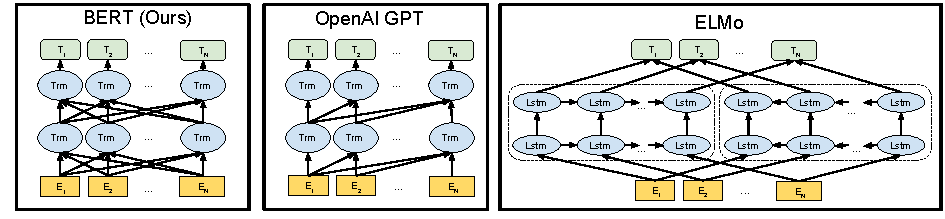
\includegraphics{figures/bert-gpt2-elmo-model-comparison}
\caption[Visualisation of the different model architectures]{Visualisation of the different model architectures \cite[p.~13]{devlin2018bert}.}
\label{fig:bert-gpt2-elmo-model-comparison}
\end{figure}

What's new about BERT, compared to other models like GPT-2, is, that it is the first deeply bidirectional language model, that takes advantage of the whole context around of a word.
OpenAI's GPT-2 uses a left-to-right Transformer \cite[p.~4]{radford2019language}, which only allows it to "look" at the words to the left, when generating a representation for an input token.
For example, when having a sentence that starts with "The lighter", the network can only look at these two words to generate a representation for the word "lighter".
However, the word can have completely different meanings, depending on the whole sentence, e.g. "The lighter is an easy tool to make fire" compared to "The lighter shade of red looks better than the darker one". 
ELMo tries to compensate this issue by training two LSTMs with one being a normal forward LSTM (left-to-right) and the other one being a backward LSTM (right-to-left) which is given the input sequence in reverse \cite[p.~2--3]{1802.05365}.
Afterwards, it concatenates the representations of these two LSTMs to get a semi-bidirectional representation.
\autoref{fig:bert-gpt2-elmo-model-comparison} visualizes the different architectures.

\subsection{Model Architecture}

\subsubsection{Input and Output Representations}

BERT's input tries to be applicable for many different natural language processing tasks.
It allows the inputs of either one sentence or a pair of two sentences, with sentences refering to ``an arbitrary span of contiguous text, rather than an actual linguistic sentence'' \cite[p.~4]{devlin2018bert}.
Texts are tokenized by using WorkPiece embeddings with a vocabulary of 30'000 tokens. % TODO Maybe explain the tokenization in more detail
Every input sequence starts with a special \texttt{[CLS]} token and every sentence ends with a special \texttt{[SEP]} token.
Additionally to the token embeddings, the input consists of two more types of embeddings.
A learned segment embeddings, that indicates if a token belongs to the first or the second token, and trained position embeddings, that help the network to understand the positions of each token in the sequence.
Finally, these three embeddings are concatendated to form the actual input for the network as shown in \autoref{fig:bert-input-representation}.

\begin{figure}[h]
\centering
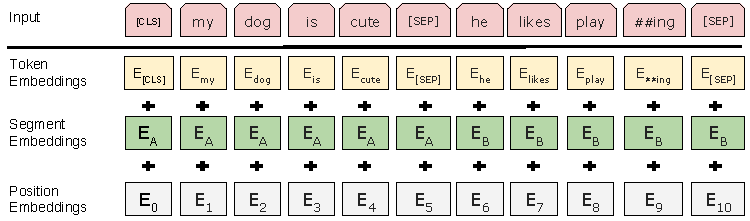
\includegraphics{figures/bert-input-representation}
\caption[BERT input representation]{BERT input representation \cite[p.~5]{devlin2018bert}.}
\label{fig:bert-input-representation}
\end{figure}

Depending on the task to perform, there are different ways to use the final hidden states of the BERT Transformer network.
For sentence classification tasks, the \texttt{[CLS]} token representation can be used.
This work uses the final hidden states for every single input token, as the Decoder should have access to the presentation of every input token.
For the simpler extractive summarization task, which is basically some kind of sentence classification in which each sentence is either classified as \texttt{"include in summary"} or \texttt{"do not include in summary"}, it can be sufficient to only use the final hidden state of the \texttt{[CLS]} token. 
\cite{1903.10318} proposes a small input variation for BERT, that inserts multiple \texttt{[CLS]} tokens into the input sequence to later use them for extractive summarization.

\subsubsection{Pre-Training Objectives}

BERT is pre-trained with two different tasks \cite[p.~4--5]{devlin2018bert}.
For the first task, the network is given a sentence with 15\% of its word piece tokens b randomly masked.
An example for masking is shown in \autoref{bert_masking_example}.

% TODO Exact source is https://github.com/google-research/bert#what-is-bert
% TODO I need to ask my prof if the current mentioning of the GitHub page is enough
\begin{lstlisting}[caption={Masked input example. Taken from the BERT GitHub page.},captionpos=b,numbers=none,label=bert_masking_example]
Input: the man went to the [MASK1] . he bought a [MASK2] of milk.
Labels: [MASK1] = store; [MASK2] = gallon
\end{lstlisting}

The task of the network is, to predict the masked tokens.
This task allows the network to take the context of a word into consideration.

For the second task, the network is given two sentences.
The network then has to predict, if the second of these two sentences comes after the first one in the original text or if it is just a randomly selected sentence from any other text.
An example for next sentence prediction is shown in \autoref{bert_next_sentence_example}.

% TODO Exact source is https://github.com/google-research/bert#what-is-bert
% TODO I need to ask my prof if the current mentioning of the GitHub page is enough
\begin{lstlisting}[caption={Next sentence prediction example. Taken from the BERT GitHub page.},captionpos=b,numbers=none,label=bert_next_sentence_example]
Sentence A: the man went to the store .
Sentence B: he bought a gallon of milk .
Label: IsNextSentence

Sentence A: the man went to the store .
Sentence B: penguins are flightless .
Label: NotNextSentence
\end{lstlisting}

Ideally, this helps the network to understand the relationship between two sentences.
However, this task has been shown to be too simple for the network, as it is easier for it to just learn if the topics of two sentences match instead of understanding the real relationship of the sentences.
Newer successors of BERT such as ALBERT use slightly changed training objectives, like sentence order prediction \cite[p.~3]{1909.11942} in which the goal is to predict, which of two given sentences comes first.

Pre-training is usually very expensive.
The training was performed for 4 days on 4 Cloud TPUs for BERT\textsubscript{BASE} and 16 Cloud TPUs for the larger model BERT\textsubscript{LARGE} with each Cloud TPU having 4 TPU chips \cite[p.~13]{devlin2018bert}.
However, it is only necessary to do pre-training once.

\subsubsection{Fine-Tuning}

After the unsupervised pre-training, the network can be fine-tuned for a specific task.
Fine-Tuning is far less expensive than pre-training and can usually be done in less than 1 hour on a single Cloud TPU, or a few hours on a normal GPU \cite[p.~5]{devlin2018bert}.
% TODO This chapter can be a bit longer...
\chapter{Used Corpora}\label{ch:used-corpora}

\Blindtext

% ==============
% AMI MEETING CORPUS
% ==============

\section{AMI Meeting Corpus}

\Blindtext

% ==============
% ICSI MEETING CORPUS
% ==============

\section{ICSI Meeting Corpus}

\Blindtext
\chapter{Concept}\label{ch:concept}

\Blindtext

% ===============
% MODEL ARCHITECTURE
% ===============

\section{Model Architecture}

\Blindtext

% =======
% TRAINING
% =======

\section{Training}

\Blindtext
\chapter{Implementation}\label{ch:implementation}

\Blindtext

% ======================
% PREPARATION OF TRAINING DATA
% ======================

\section{Preparation of Training Data}

\Blindtext

\subsection{NXT}

\Blindtext

\subsection{Data Cleaning}

\Blindtext

\subsection{Data Split}

\Blindtext

% ===================
% IMPLEMENTATION WITH TEXAR
% ===================

\section{Implementation with Texar}

\Blindtext

% ===================
% TRAINING HYPERPARAMETERS
% ===================

\section{Training Hyperparemeters}

\Blindtext
\chapter{Results}\label{ch:results}

\Blindtext

% =======
% FIRST STEP
% =======

\section{First Step}

\Blindtext

% =========
% SECOND STEP
% =========

\section{Second Step}

\Blindtext

\chapter{Outlook}\label{ch:outlook}

\Blindtext
\chapter{Summary and Conclusion}\label{ch:summary-and-conslusion}

\Blindtext

\backmatter
\listoffigures
\cleardoublepage

\listoftables
\cleardoublepage

\renewcommand{\lstlistlistingname}{List of Listings}  % change for German thesis
\lstlistoflistings
\cleardoublepage

\bibliographystyle{wmaainf}
\bibliography{refs}

\end{document}
